\section{Input Power Quality}
\label{sec:res-pq}

The high-power \SI{20}{\volt} records gave the best logged input power quality.
Between \SI{3.7}{\ampere} and \SI{4}{\ampere}, PF approached unity and
current THD was lower than at several low-power points
(Figure~\ref{fig:rebuilt-pq}).

\begin{figure}[htbp]
\centering
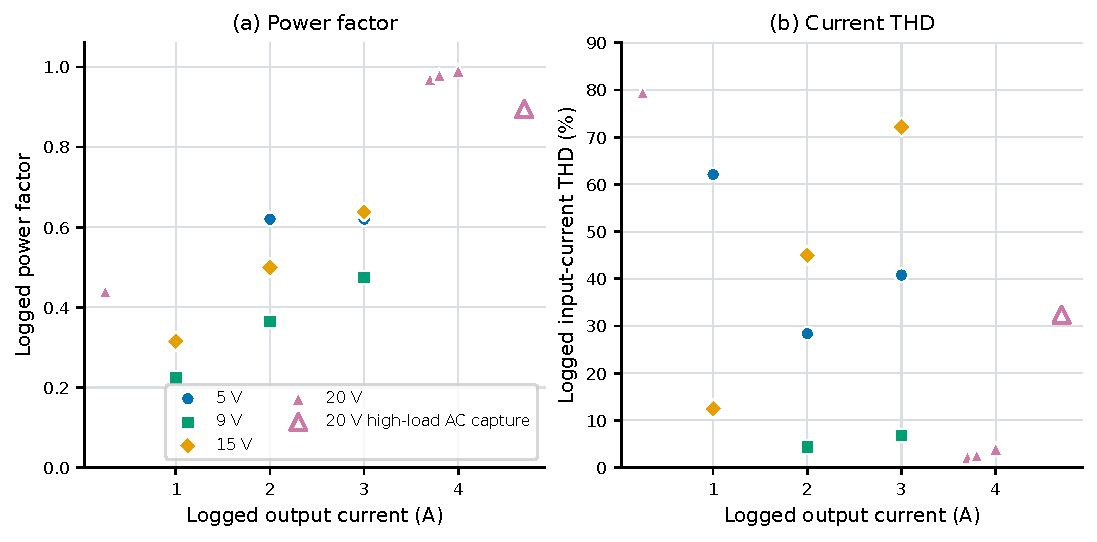
\includegraphics[width=\textwidth]{Pictures/Thesis/10_Results/Rebuilt/power_quality.pdf}
\caption{Measured input PF and current THD versus load. Filled markers use DC-coupled output measurements; the open marker is the \SI{4.7}{\ampere} test with AC-coupled output channels. Some PF and THD readings come from different instruments. Only measured points are shown.}
\label{fig:rebuilt-pq}
\end{figure}

For a common averaging interval, power factor is
\begin{equation}
\mathrm{PF}=\frac{P_\mathrm{in}}{V_\mathrm{in,rms}I_\mathrm{in,rms}},
\end{equation}
and current THD is
\begin{equation}
\mathrm{THD}_I=
\frac{\sqrt{\sum_{n=2}^{N}I_{n,\mathrm{rms}}^2}}
{I_{1,\mathrm{rms}}}\,100\%.
\end{equation}
The logged readings are plotted directly. Some rows combine Siglent PF and
ITECH THD from separate captures. Those readings cannot be used together to
calculate displacement factor.

At \SI{20}{\volt}, the \SI{3.7}{\ampere}, \SI{3.8}{\ampere}, and
\SI{4.0}{\ampere} tests give PF of 0.97, 0.98, and 0.99, with current
THD of \SI{2.23}{\percent}, \SI{2.62}{\percent}, and
\SI{3.98}{\percent}. The \SI{3.9}{\ampere} point was omitted from
the trend because its power-quality entries repeat an associated measurement
set.
The \SI{4.7}{\ampere} capture gives Siglent PF 0.894 and ITECH THD
\SI{32.42}{\percent}, with an earlier firmware revision identified in Table~\ref{tab:prototype-identity}. The
difference includes changed firmware and measurement conditions as well as
load; it cannot be attributed to load alone.

\begin{figure}[htbp]
\centering
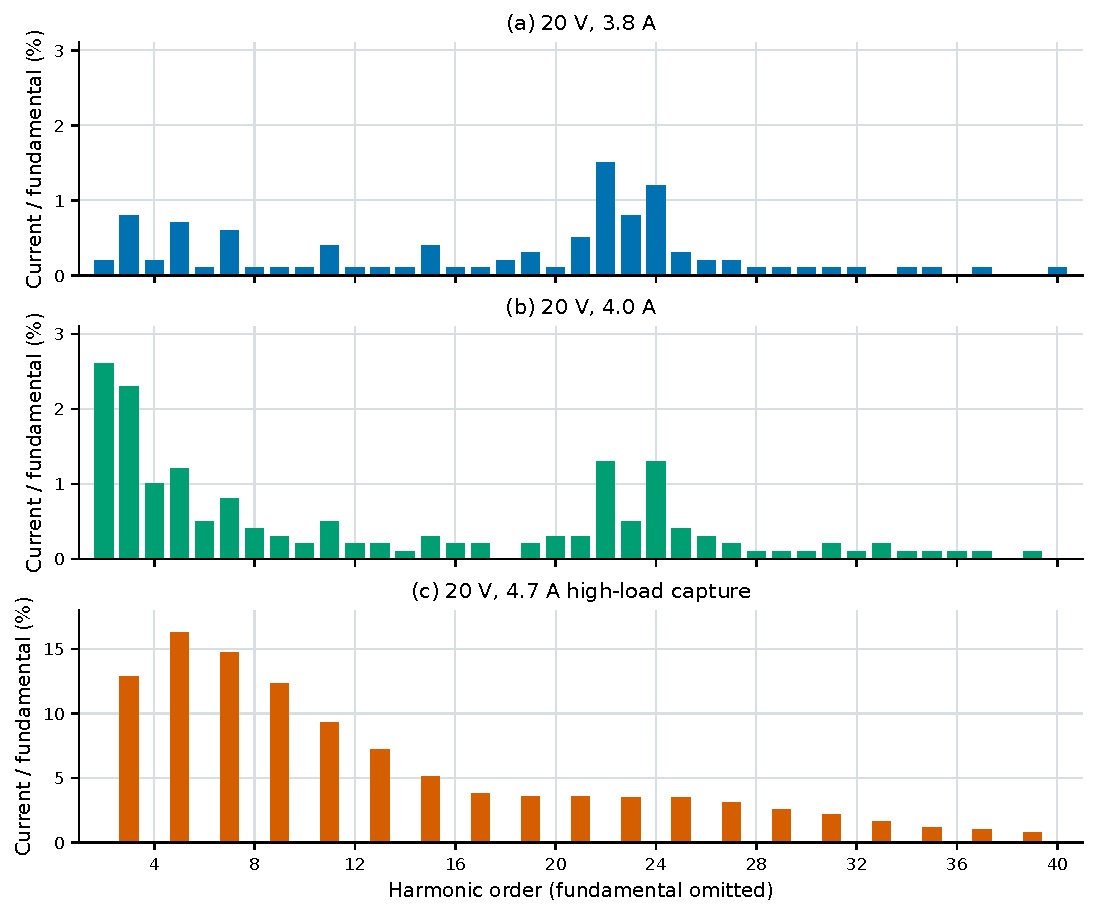
\includegraphics[width=0.96\textwidth]{Pictures/Thesis/10_Results/Rebuilt/current_harmonic_spectrum.pdf}
\caption{Normalized input-current harmonic spectra transcribed from the original ITECH tables at \SI{3.8}{\ampere}, \SI{4.0}{\ampere}, and the \SI{4.7}{\ampere} high-load setting. The fundamental is omitted for readability. The upper panels use a 0--3.1\% scale; the lower panel uses a 0--18\% scale. All orders 1--40 are included in Table~\ref{tab:input-harmonics}.}
\label{fig:rebuilt-harmonic-spectrum}
\end{figure}

At \SI{3.8}{\ampere},
the largest listed component above the fundamental is the 22nd harmonic at
\SI{1.5}{\percent}. At \SI{4.0}{\ampere}, the second and third are
\SI{2.6}{\percent} and \SI{2.3}{\percent}. At \SI{4.7}{\ampere}, the
third, fifth, seventh, and ninth dominate at \SI{12.9}{\percent},
\SI{16.3}{\percent}, \SI{14.7}{\percent}, and \SI{12.3}{\percent}
of the fundamental. Screenshot-checked components through order 40 give
root-sum-square THD values of
approximately \SI{2.64}{\percent}, \SI{4.53}{\percent}, and
\SI{32.49}{\percent}. At \SI{4.0}{\ampere}, the reconstructed result
and separate \SI{3.98}{\percent} screen differ by more than table rounding.
The discrepancy remains unresolved; both values are retained pending a
synchronized repeat.

\begin{figure}[htbp]
\centering
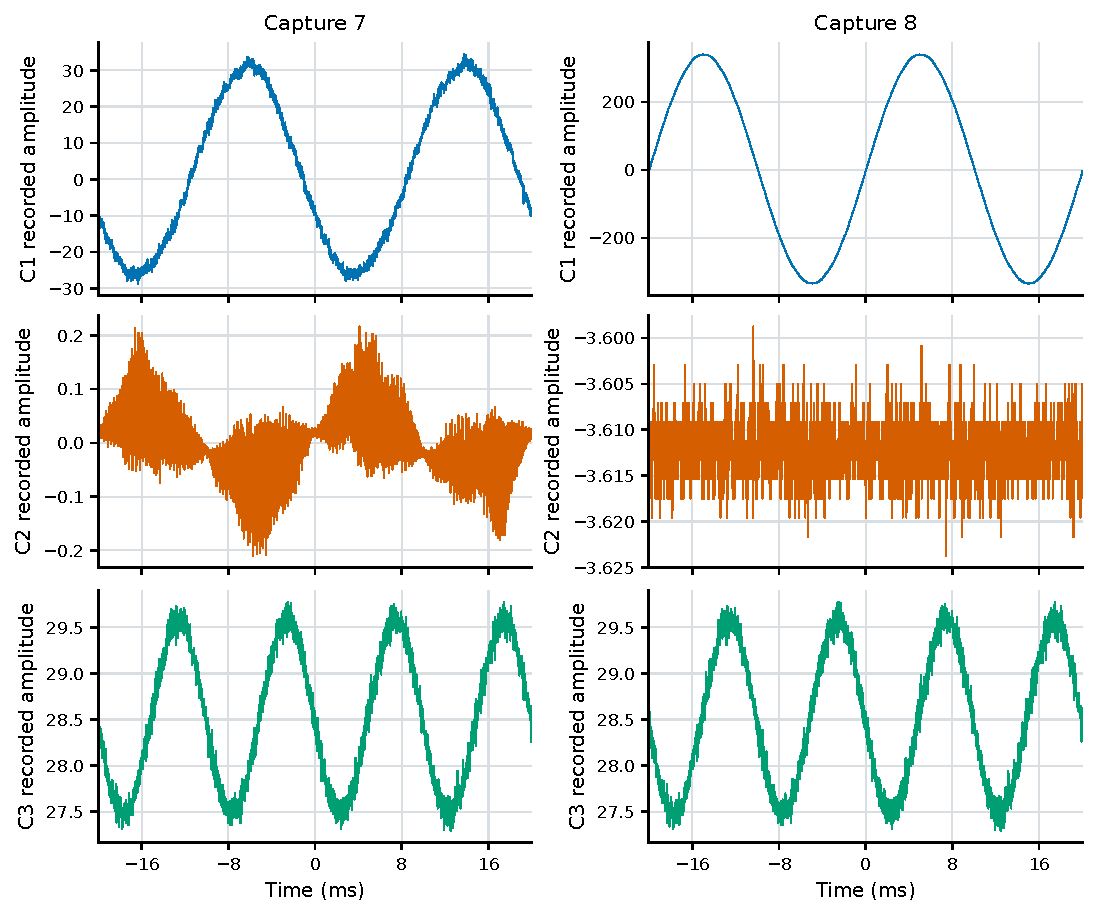
\includegraphics[width=\textwidth]{Pictures/Thesis/10_Results/Rebuilt/raw_line_records.pdf}
\caption{LeCroy line-timescale waveforms from captures 7 and 8. The two C3 records contain identical data.}
\label{fig:rebuilt-raw-line}
\end{figure}

The line-timescale traces show the input waveform, but incomplete probe
calibration prevents calculation of PF or real power from them.

Earlier charge-pump results \cite{ammar2020chargepump,ammar2021led} used
different operating conditions. Input filtering, magnetics, output setting,
and burst structure differ from this prototype. Table~\ref{tab:pq-results} retains the full
readings and identifiers.
